% CREATED BY DAVID FRISK, 2018
\chapter{Results and Discussions}

\begin{table}[h]
    \centering
    \begin{tabular}{|c|c|c|c|c|}
        \hline
        Dataset & Mean LT (px) & LT Variance (px) & Mean Accuracy & Mean entropy\\
        \hline
        MNIST test & 1.48 & 0.126 & 0.98 & 0.024\\
        \hline
        CTHMNIST & 1.38 & 0.21 & 0.87 & 0.106\\
        \hline
    \end{tabular}
    \caption{Comparisons of basic attributes of CTHMNIST and the MNIST test set. The Line Thickness (LT) are calculated using the methods described by \cite{kozielski2012moment}. The line thicknesses are calculated using 28 by 28 images. The CTHMNIST digits are preprocessed just using the procedure decribed in \cite{lecunmnist}. The mean entropy is calculated by averaging the entropy of each digits that were fed to the network. Both the mean accuracy and mean entropy in this table are calculated by averaging the results over 20 independent trials}
    \label{tab:datasets}
\end{table}

\section{Comparison of MNIST and CTHMNIST}

Table \ref{tab:datasets} shows the calculated line thickness of both the MNIST test set and CTHMNIST digits in their 28-by-28 dimensions. Without applying any kind of line thickness manipulation or normalization, the results in table \ref{tab:datasets} demonstrates the difference some difference in attributes. At least from what can be observed, based on the lower accuracy and higher entropy is that the digits in the CTHMNIST dataset is harder to classify for a single CNN using. The higher mean entropy observed here vaguely indicates that there is a correlation between entropy and classification error.

Figure \ref{fig:digitscomp} samples of the numbers 6,9,4, and 7 from both datasets. From what we can see, there is no clear differences between these samples. Though we do see that the MNIST samples in fig \ref{fig:digitscomp} contains more grey scale pixels then those from CTHMNIST.

\begin{figure}[h]
    \centering
    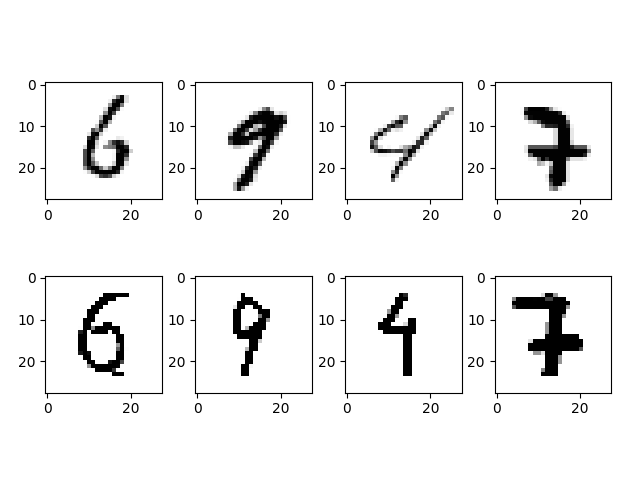
\includegraphics[scale=0.9]{figure/digitscompare.png}
    \caption{Samples of both the MNIST test set and CTHMNIST. The top row are samples from the MNIST test set and the bottom row consist of samples from CTHMNIST of the same numbers.}
    \label{fig:digitscomp}
\end{figure}
\newpage
\section{Distortions using Line Thickness}

Figure \ref{fig:mlpensemble} shows the classification error and average information entropy (entropy averaged over the input) of ensembles in the size of 5,20,50, and 100 are plotted as a function of Line thickness. We observe that increasing the ensemble size past that of 20 does not significantly improve nor deteriorate classification error. Rather, the metric seems to have converged as the ensemble size increases past 20. When looking at the plot of entropy (right panel of fig. \ref{fig:mlpensemble}) we observe that entropy seems to be increasing with ensemble size. However just like in the case of classification error, the increase in entropy as a function of ensemble size seems to have converged when the ensemble sizes goes past the size of 20. This results is consistent with the observations reported by \cite{lakshminarayanan2017simple}.

The resulting images of line thickness manipulations using \cite{kozielski2012moment} can be seen in Figure \ref{fig:digits}. From this figure observe that while the image of 4 continues to be fairly recognizable at the line thickness of 30, both 8 and 9 have started to lose their shape at the same line thickness as 4. From the results in figure \ref{fig:digits}, we can see that Both 8 and 9 are starting lose their charactaristic pelletings at high line thickness. Incidentally, we can also observe that the independent dots in the images have started to merge with the digits at a certain line thickness. 

\begin{figure}[t]
    \centering
    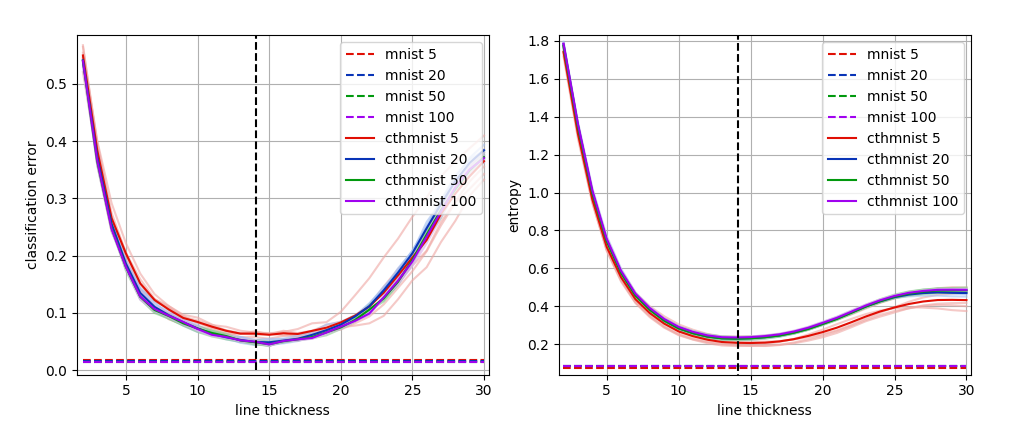
\includegraphics[scale=0.6]{figure/mlpensemble.png}
    \caption{The classification error and entropy Deep ensemble consisting of Multi layered perceptrons of size 5, 20, 50, and 100. The left panel plots the classifcation error as a function of line thickness, the right panel plots the average entropy over the mutated  CTHMNIST dataset as a function of Line thickness. These results are produced over 5 independent trials. Here the darker lines represents the average over the runs, while the lighter lines shows the different fluctuations from each run. The horizontal dashed lines are the average classification error and average entropy respctively over the trials for the MNIST test set, and the vertical black dashed line is an approximated average line thickness of the MNIST test set scaled up to that of 280-by-280}
    \label{fig:mlpensemble}
\end{figure}

\begin{figure}[h!]
    \centering
    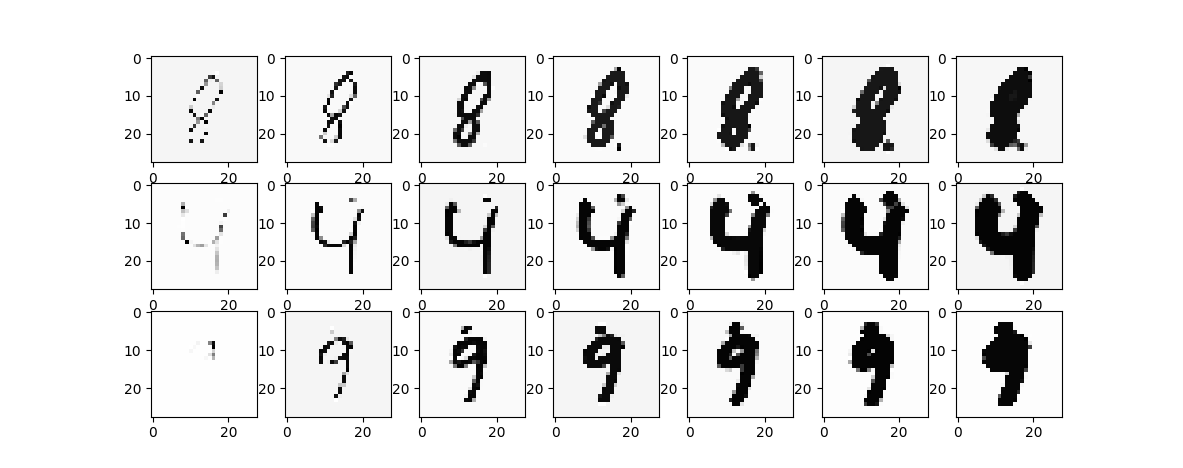
\includegraphics[scale = 0.5]{figure/digits.png}
    \caption{The change of sample images of an 8,4 and a 9 over line thicknesses. The columns are ordered by Linethickness. Starting from the left most columns, the figure illustrates these same images adjusted to the line thicknesses in the order 2, 5, 10, 15, 20, 25, and 30}
    \label{fig:digits}
\end{figure}

\begin{figure}
    \centering
    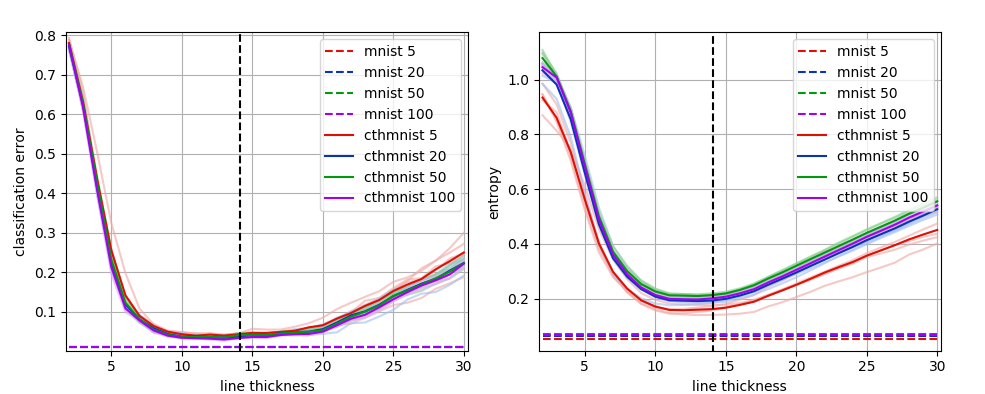
\includegraphics[scale=0.6]{figure/cnnEnsemble.png}
    \caption{Classification error and average entropy of ensembles consisting of CNNs. This figure illustrates the results from running the same experiment that produces \ref{fig:mlpensemble} using CNNs instead of multi layered perceptron. The rest of the settings for this figure remains the same as \ref{fig:mlpensemble}.}
    \label{fig:cnnensemble}
\end{figure}

The previously described observations with regards to convergence of our metrics with regards to ensemble size is also observed in the case of ensembles of CNN as seen in figure \ref{fig:cnnensemble}. A common observation in both \ref{fig:mlpensemble} and \ref{fig:cnnensemble} is that their seems to be a strong correlation between mean entropy and classification error as both of these metrics seems to increase and decrease in similar ways. Interestingly when comparing \ref{fig:cnnensemble} to \ref{fig:mlpensemble}, we can see that the classification seems to form a plateau over the line thicknesses between 10 and 20. 

\subsection{Individual networks vs Ensemble}
\begin{figure}
    \centering
    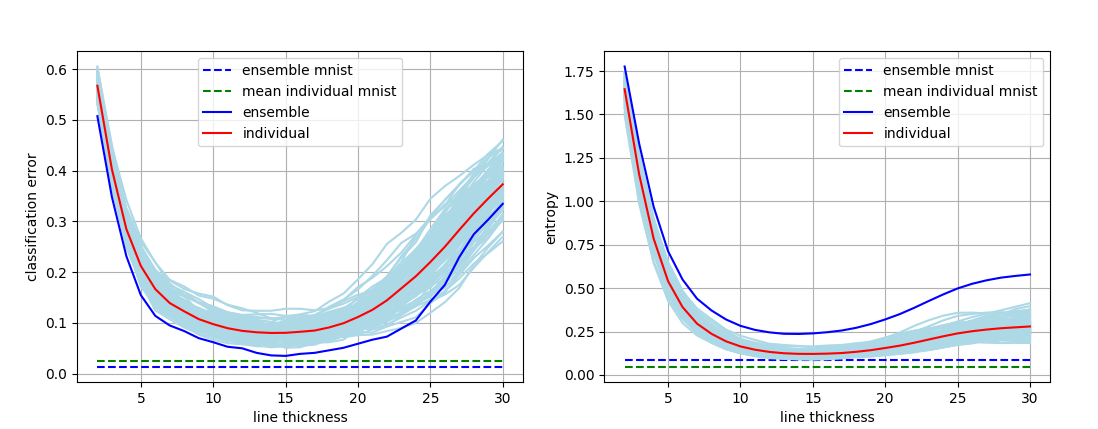
\includegraphics[scale=0.55]{figure/EnsembleVsIndividual.png}
    \caption{Performance comparison between individual Multi-layer Perceptron classifiers and an ensemble of 100 MLPs. The left panel plots the classification error as a function of line thickness, and the right panel plots the Average entropy over the CTHMNIST dataset.In both panels, lightblue colored lines represent the results of individual MLP classifiers over 100 trials. This is compared to the darker blue line which corresponds to the results produced by a size 100 ensemble during 1 single trial. The red lines represents the average performance of each individual ANN at each line thickness.}
    \label{fig:mlpvsensemble}
\end{figure}

\begin{figure}
    \centering
    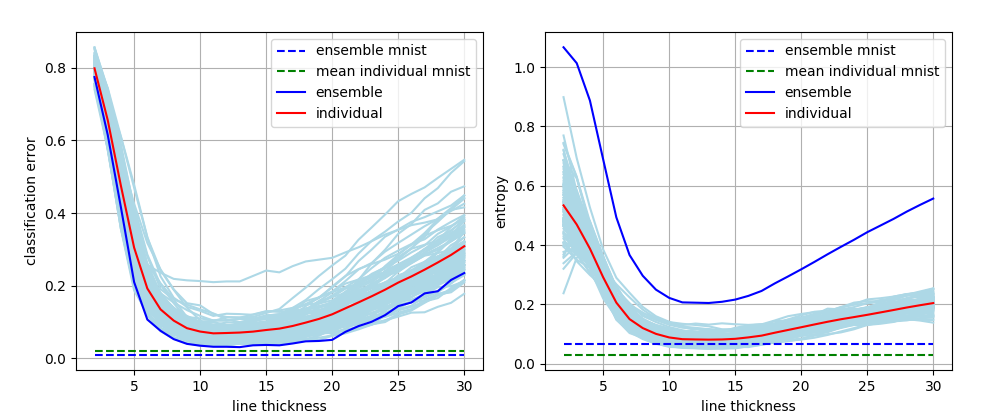
\includegraphics[scale=0.6]{figure/CNNEnsembleVsIndividual.png}
    \caption{Same experiments as figure \ref{fig:mlpvsensemble}, produced with CNNs and ensemble of CNNs instead MLPs}
    \label{fig:CNNvsensemble}
\end{figure}

\subsection{Effect of Adversarial training}
\begin{figure}
    \centering
    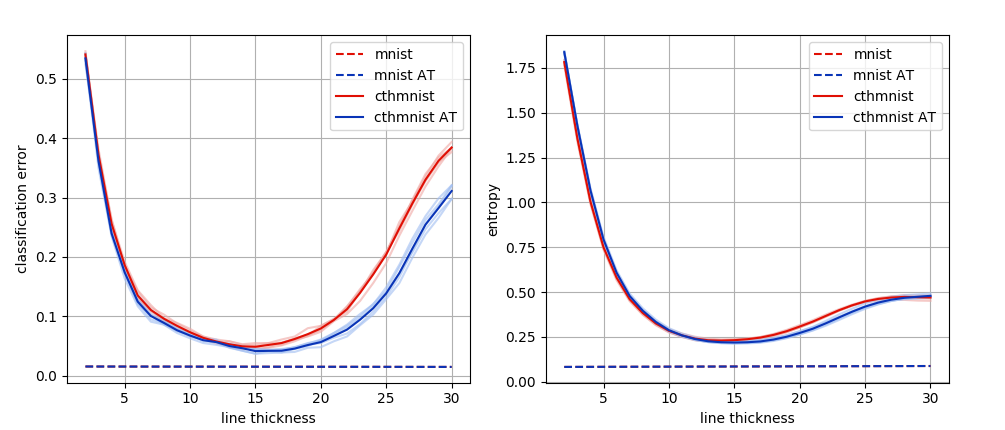
\includegraphics[scale=0.6]{figure/ATvsNoAT.png}
    \caption{Comparisons of between two size 20 ensembles of MLPs where one is trained using Adversarial Training, These results are produced over 5 independent trials. Once again, the darker colored lines are the average over these independent runs, and the lighter once are the fluctuations.}
    \label{fig:AT}
\end{figure}

\subsection{Voting compared to averaging}
\begin{figure}
    \centering
    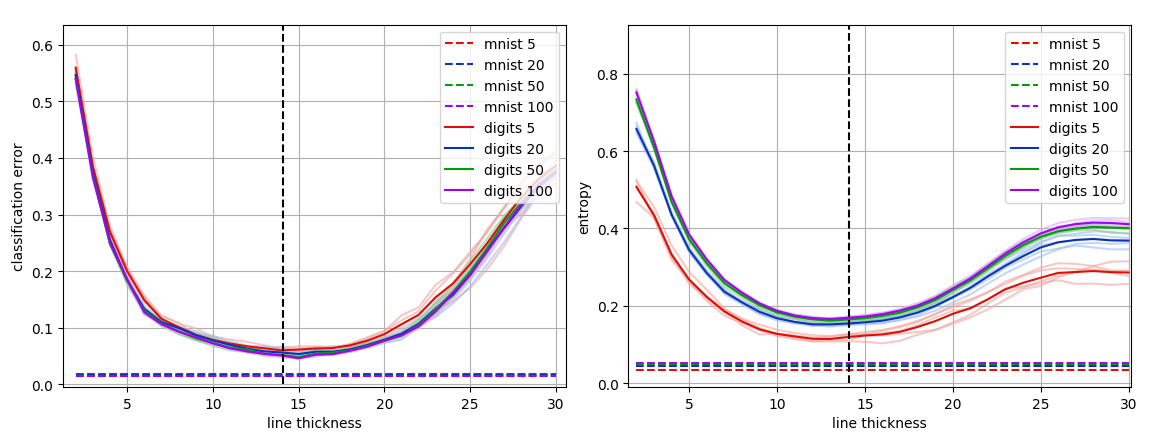
\includegraphics[scale=0.5]{figure/ensembleVote.png}
    \caption{The results from using an ensemble that uses member voting instead of Averaging the member predictions.}
    \label{fig:vote}
\end{figure}

\section{Salt and pepper noise.}

\begin{figure}
    \centering
    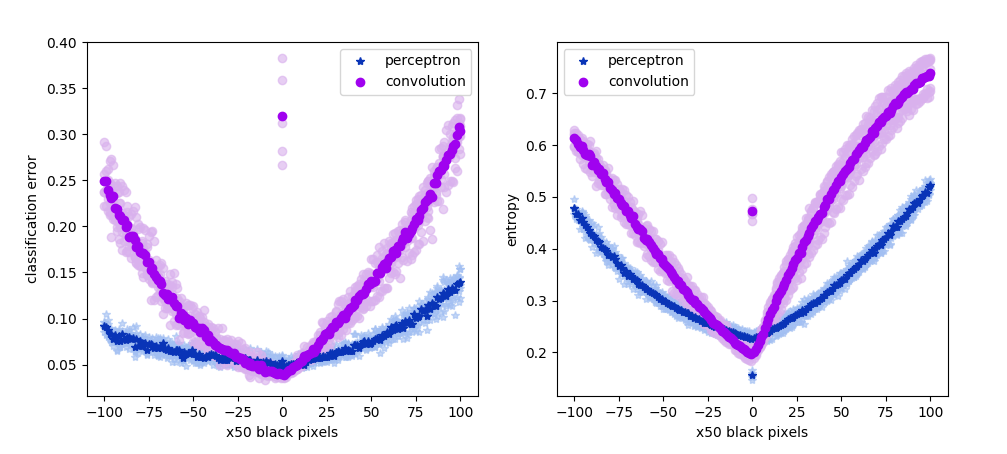
\includegraphics[scale=0.6]{figure/trippySaltnPepper.png}
    \caption{Classification error and entropy produced by 2 ensembles over 5 trials each with the inputs distorted with salt and pepper noise. One ensemble consist of MLPs, and the second consist of CNNs. The noise is applied to the digits adjusted to that of line thickness with least classification error. Based previous observed results from figure \ref{fig:digits}, this line thickness is 14. The noise is applied by first selecting a number of black pixels, turning them white, and then from the unmodified image, choosing a number of white pixels turning them black. Each step on the x-axis corresponds to a multiple of 50 pixels.}
    \label{fig:saltpepper1}
\end{figure}

\begin{figure}
    \centering
    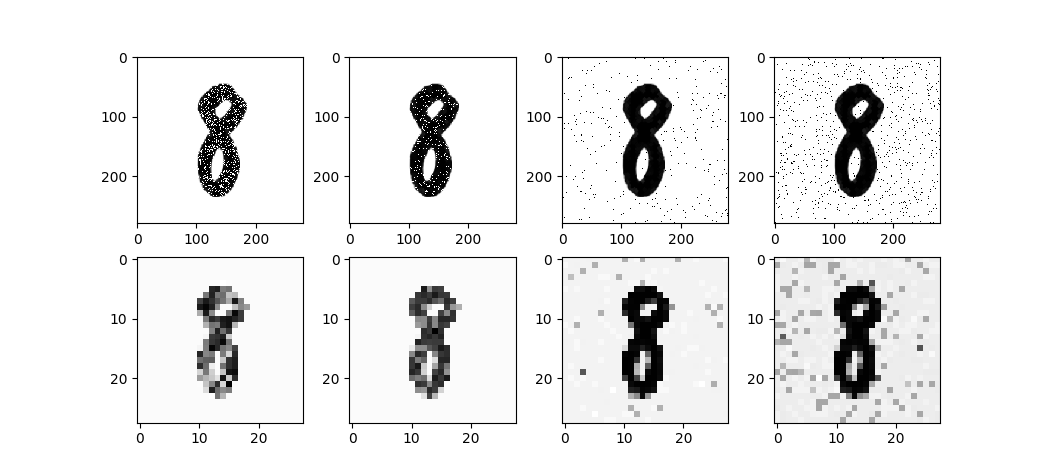
\includegraphics[scale=0.5]{figure/digitsSaltnpepper.png}
    \caption{Images of an 8 Distorted with salt and pepper noise applied the same way it's described in figure \ref{fig:saltpepper1}. The first row is the 280-by-280 sized image of the digits just after the noise is applied. Bottom row images are the results of scaling down the images to 28-by-28, which is the images given to NN classifiers. The left most and right most columns corresponds to removing resp. adding 2000 black pixels, and the middle left, and middle right columns corresponds to removing resp. adding 800 black pixels}
    \label{fig:digitssaltandpepper}
\end{figure}

\begin{figure}
    \centering
    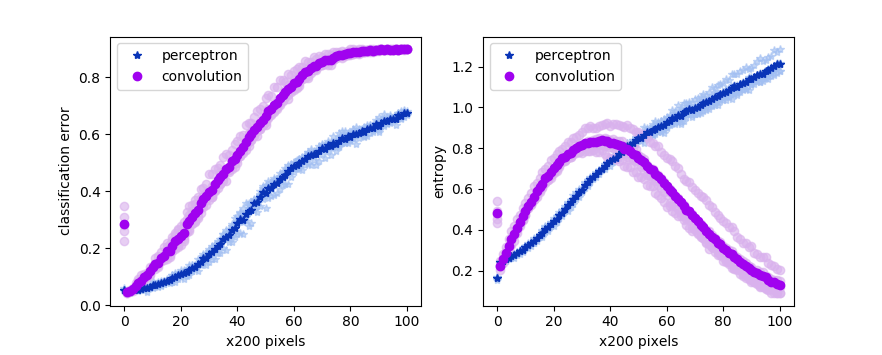
\includegraphics[scale=0.7]{figure/trippySaltnPepperOPT.png}
    \caption{Classification error and average entropy produced by an ensemble of CNNs and an ensemble of MLPs with inputs distorted with Salt and pepper noise. The noise is applied by randomly selecting a number of pixels and flipping their values. The randomly selected white pixels turns black and the black pixels turns white. In this plot, the noise is applied to CTHMNIST digits adjusted to line thickness with least classification error. The darker markers represents the average over the trials and the lighter ones represent the fluctuations over the trials}
    \label{fig:saltpepper2}
\end{figure}

\begin{figure}
    \centering
    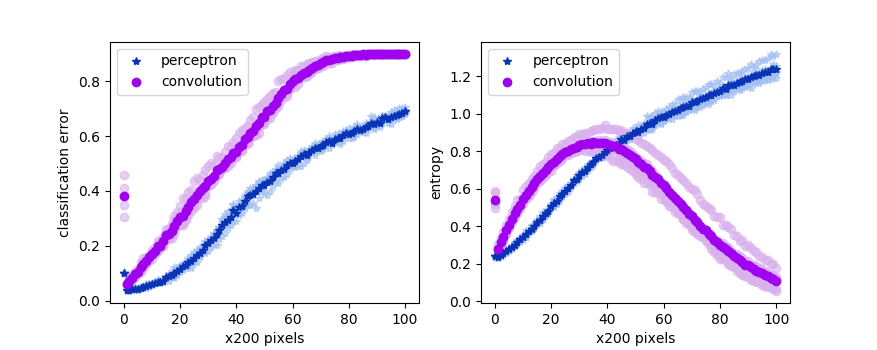
\includegraphics[scale=0.7]{figure/trippySaltnPepperLecunn.png}
    \caption{Results from the same experiments as figure \ref{fig:saltpepper2}. The difference here is that the noise is applied to the unmodified CHTMNIST digits rather then the once adjusted to optimal line thickness.}
    \label{fig:saltpepper2b}
\end{figure}

\begin{figure}
    \centering
    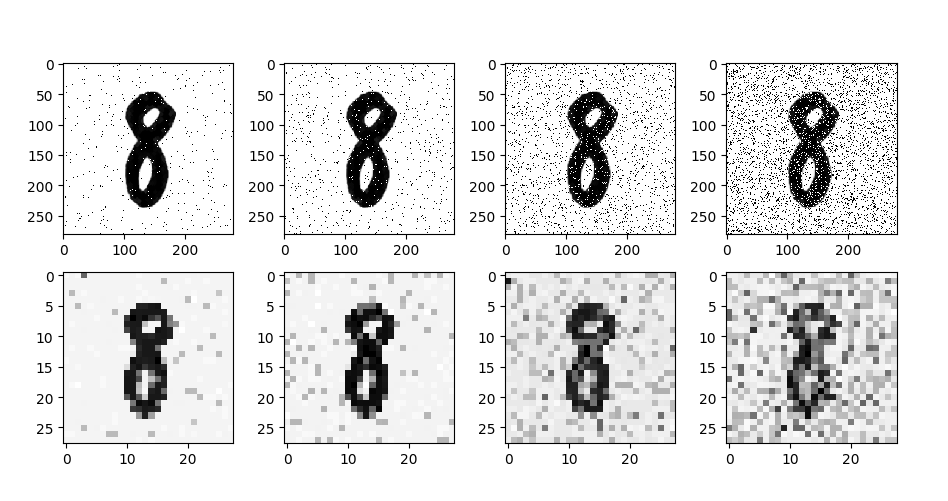
\includegraphics[scale=0.5]{figure/digitsSaltnpepper2.png}
    \caption{Images of an 8 Distorted with applied salt and pepper noise. the image. The noise is applied the same way as those that gave the results for figure \ref{fig:saltpepper2} and \ref{fig:saltpepper2b}. The sorted according to the number of pixels that were selected to flip their values. From the left, the number of pixels in each column is 1000, 2000, 5000, 10000}
    \label{fig:digitssaltandpepper}
\end{figure}

\section{Predictive uncertainty and incorrect decisions}

\begin{figure}
    \centering
    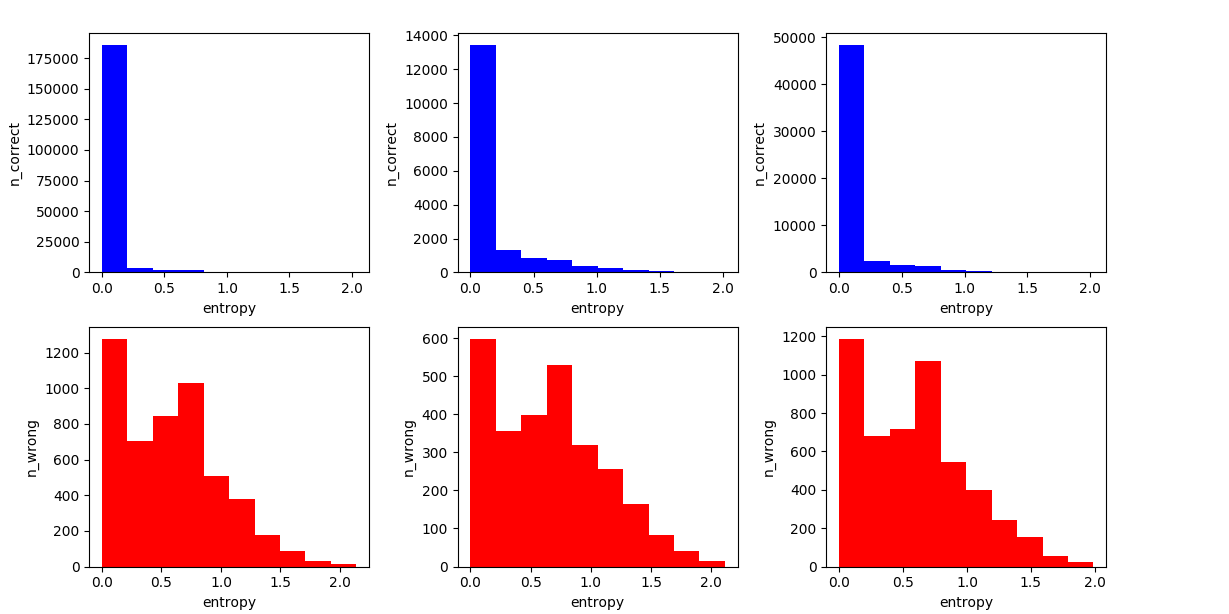
\includegraphics[scale = 0.53]{figure/EntropyFrekIndividual.png}
    \caption{Histogram of Information entropy distribution of correctly and incorrecly classified datapoints. The blue histograms corresponds to correctly classified input and the red ones are incorrecly classified inputs. These values are produced by using a single multi-layer perceptron classifier. The left most column is produced using the MNIST testset, center column CTHMNIST without any adjustments to line thickness, and the right one is produced using the CTHMNIST digits adjusted to the vicinity of optimal Line thickness, which ranges from 13-15.}
    \label{fig:hist1mlp}
\end{figure}

\begin{figure}
    \centering
    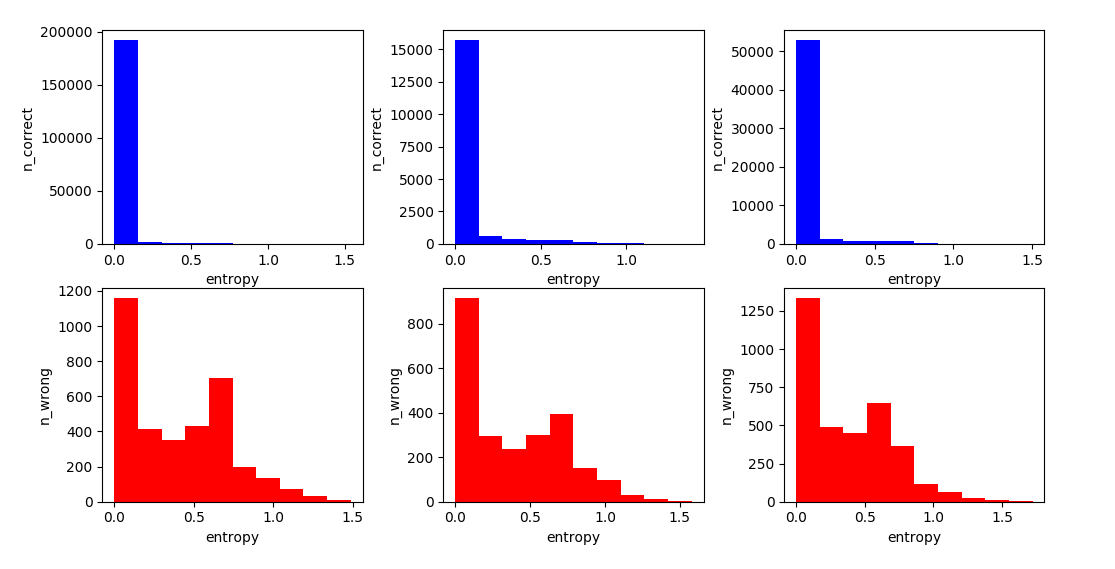
\includegraphics[scale=0.55]{figure/CNNEntropyFrekIndividual.png}
    \caption{Same histograms as in figure \ref{fig:hist1mlp}. This one is produced using a single convolutional neural network trained using MNIST.}
    \label{fig:hist1cnn}
\end{figure}

\begin{figure}
    \centering
    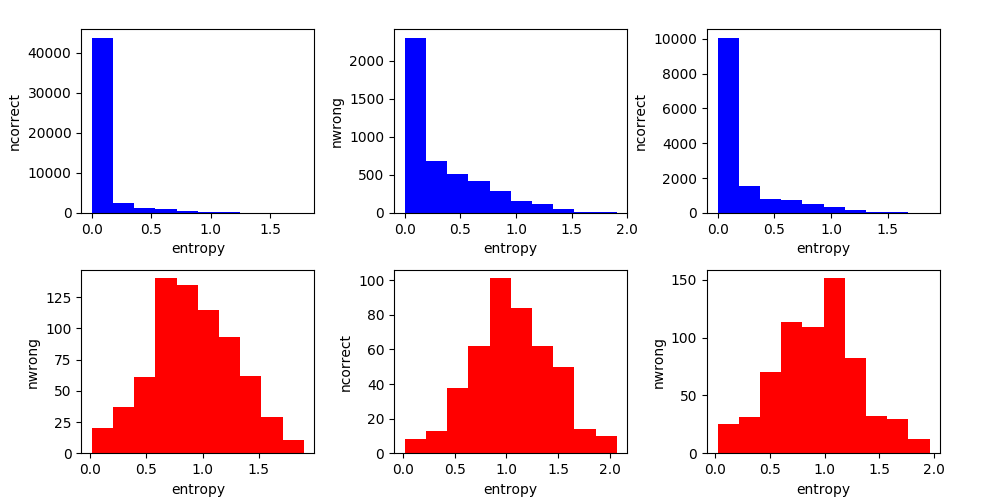
\includegraphics[scale=0.6]{figure/EntropyFrekEnsemble.png}
    \caption{The experiments from figure \ref{fig:hist1mlp} and \ref{fig:hist2mlp}, but performed using an ensemble of 20 multi-layer perceptrons. }
    \label{fig:hist2mlp}
\end{figure}


\begin{figure}
    \centering
    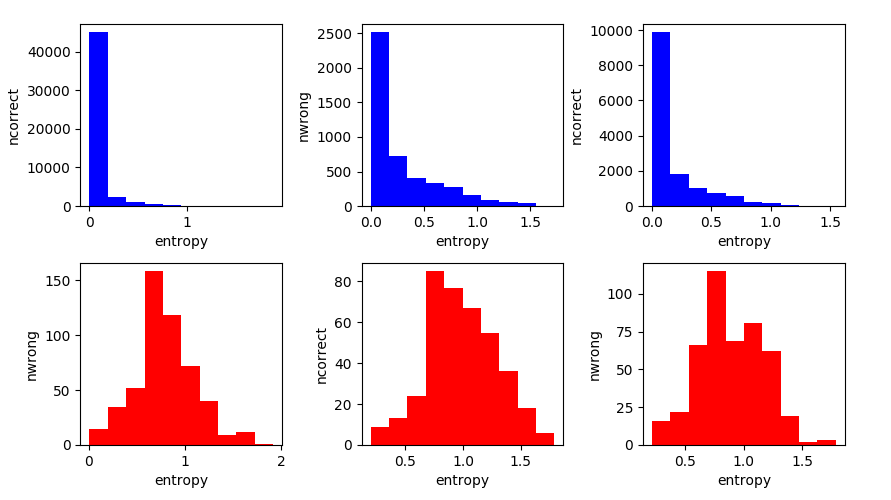
\includegraphics[scale=0.7]{figure/CNNEntropyFrekEnsemble.png}
    \caption{The experiments from figure \ref{fig:hist1mlp} and \ref{fig:hist2mlp}, but performed using an ensemble of 20 CNNs. }
    \label{fig:hist2cnn}
\end{figure}

\begin{figure}
    \centering
    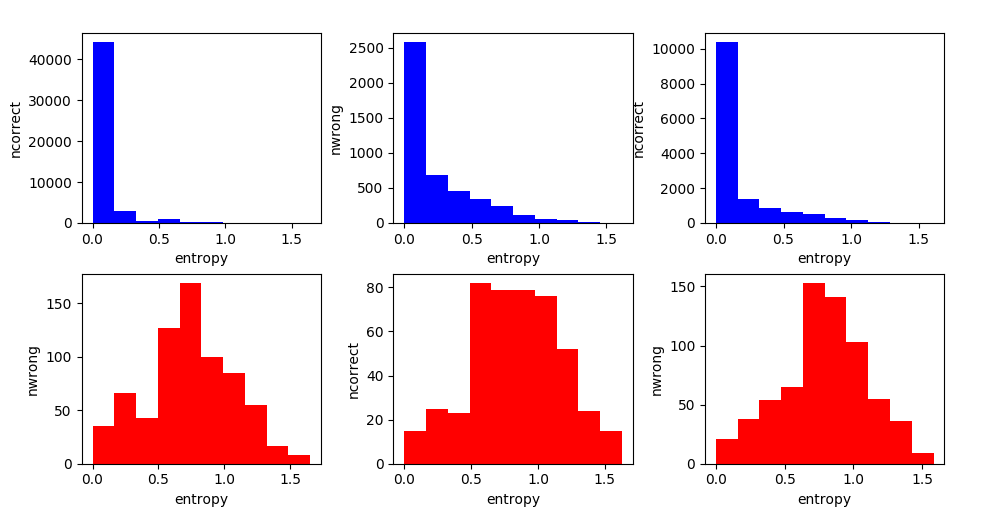
\includegraphics[scale=0.6]{figure/EntropyFrekEnsembleVote.png}
    \caption{Histograms from the same experiments that produced the previous figures, this time using a 20 member MLP ensemble that uses voting rather than prediction averaging.}
    \label{fig:hist3vote}
\end{figure}

\begin{figure}
    \centering
    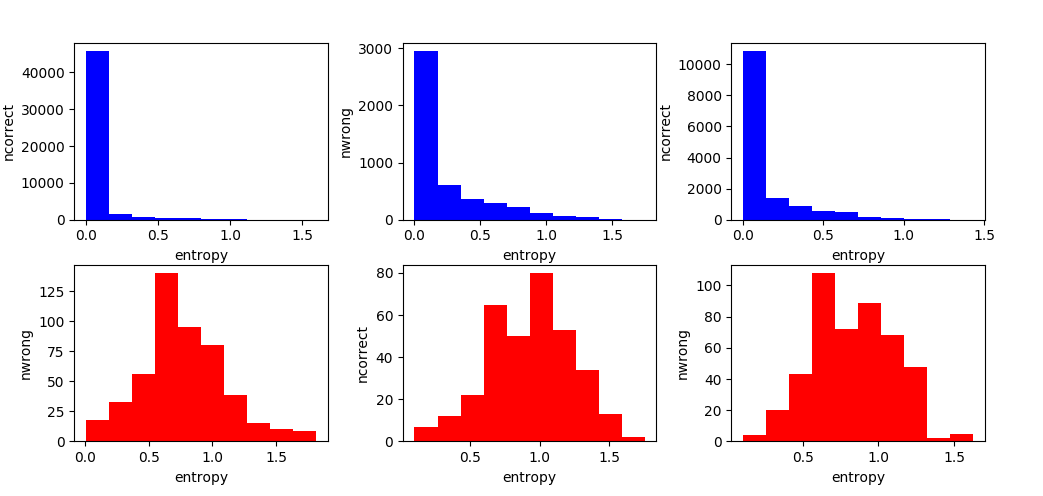
\includegraphics[scale=0.6]{figure/EntropyFrekIndividualAT.png}
    \caption{Histograms of the distribution of entropy like in the previous figures. This figure is produced using ensembles of MLPs trained using adversarial training.}
    \label{fig:hist3at}
\end{figure}

\begin{figure}
    \centering
    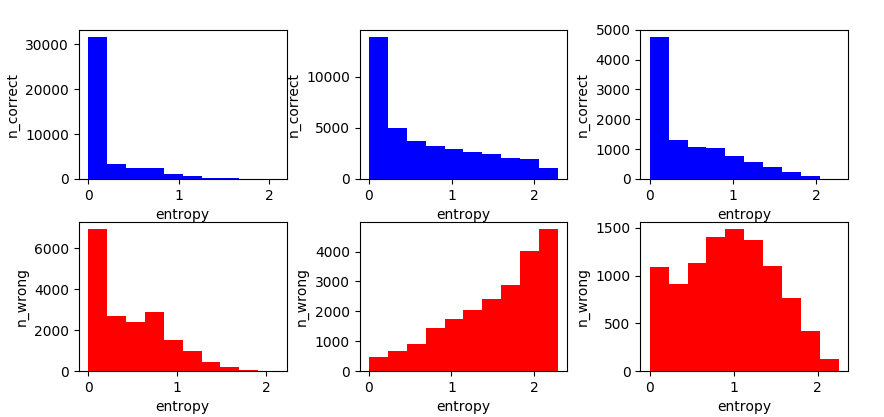
\includegraphics[scale=0.65]{figure/histHighEntropy.png}
    \caption{Histogram of the distribution of Entropy of heavily distorted inputs. The left column represents the entropy distribution of the CTHMNIST dataset with high line thickness(between 26 and 30), the center column with low line thickness (between 2 and 6) and the third column is made with CTHMNIST with salt and pepper noice with 12000 pixels flipped in the dimensions of 280-by-280. These distributions is produced by a single MLP classifier over 20 trials}
    \label{fig:hist4}
\end{figure}

\begin{figure}
    \centering
    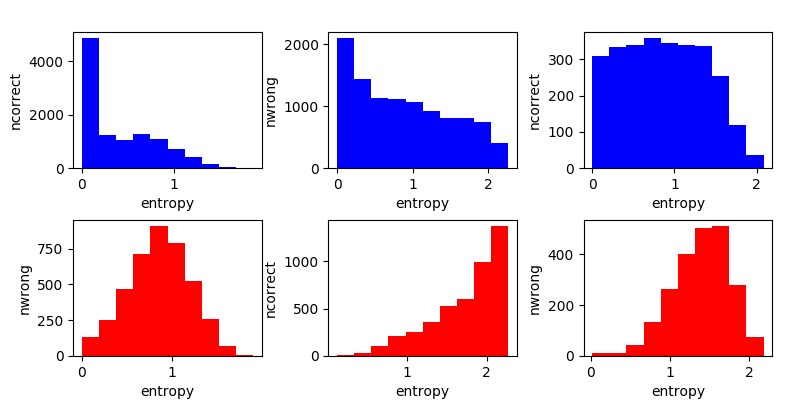
\includegraphics[scale=0.7]{figure/histHighEntropyEnsemble.png}
    \caption{Histogram using the same datasets as \ref{fig:hist4}, produced over 5 trials using an ensemble of 20 MLPs instead of a single neural network. The columns remains in the same order as they were in \ref{fig:hist4}}
    \label{fig:hist4ensemble}
\end{figure}